%%%%%%%%%%%%%%%%%%%%%%%%%%%%%%%%%%%%%%%%%
% Masters/Doctoral Thesis 
% LaTeX Template
% Version 2.1 (2/9/15)
% 
%
% This template has been downloaded from:
% http://www.LaTeXTemplates.com
%
% Version 2.0 major modifications by:
% Vel (vel@latextemplates.com)
%
% Original authors:
% Steven Gunn  (http://users.ecs.soton.ac.uk/srg/softwaretools/document/templates/)
% Sunil Patel (http://www.sunilpatel.co.uk/thesis-template/)
%
% License:
% CC BY-NC-SA 3.0 (http://creativecommons.org/licenses/by-nc-sa/3.0/)
%
%%%%%%%%%%%%%%%%%%%%%%%%%%%%%%%%%%%%%%%%%

%----------------------------------------------------------------------------------------
%	PACKAGES AND OTHER DOCUMENT CONFIGURATIONS
%----------------------------------------------------------------------------------------

\documentclass[
11pt, % The default document font size, options: 10pt, 11pt, 12pt
%oneside, % Two side (alternating margins) for binding by default, uncomment to switch to one side
spanish, % ngerman for German
singlespacing, % Single line spacing, alternatives: onehalfspacing or doublespacing
%draft, % Uncomment to enable draft mode (no pictures, no links, overfull hboxes indicated)
%nolistspacing, % If the document is onehalfspacing or doublespacing, uncomment this to set spacing in lists to single
%liststotoc, % Uncomment to add the list of figures/tables/etc to the table of contents
%toctotoc, % Uncomment to add the main table of contents to the table of contents
%parskip, % Uncomment to add space between paragraphs
]{MastersDoctoralThesis} % The class file specifying the document structure

\usepackage[utf8]{inputenc} % Required for inputting international characters
\usepackage[T1]{fontenc} % Output font encoding for international characters

\usepackage{palatino} % Use the Palatino font by default

\usepackage[backend=bibtex,style=alphabetic,natbib=true]{biblatex} % User the bibtex backend with the authoryear citation style (which resembles APA)
\addbibresource{example.bib} % The filename of the bibliography
\usepackage[autostyle=true]{csquotes} % Required to generate language-dependent quotes in the bibliography
\usepackage{graphicx}
\usepackage{caption}
\usepackage{subcaption}

\usepackage{float}
\usepackage{enumerate}
\LetLtxMacro\itemold\item
\renewcommand{\item}{\itemindent1cm\itemold}


%----------------------------------------------------------------------------------------
%	THESIS INFORMATION
%----------------------------------------------------------------------------------------

\thesistitle{Segmentación del árbol vascular de la retina en angiografías con fluoresceína} % Your thesis title, this is used in the title and abstract, print it elsewhere with \ttitle
\supervisorfirst{Dra. Mariana \textsc{del Fresno}}
\supervisorsecond{Ing. José Ignacio \textsc{Orlando}}
% Your supervisor's name, this is used in the title page, print it elsewhere with \supname
\examiner{Nombres de los jurados} % Your examiner's name, this is not currently used anywhere in the template, print it elsewhere with \examname
\degree{Ingeniero de Sistemas} % Your degree name, this is used in the title page and abstract, print it elsewhere with \degreename
\author{\\Mauro  \textsc{Giamberardino} \\ Ariel  \textsc{Borthiry} \\} % Your name, this is used in the title page and abstract, print it elsewhere with \authorname
\addresses{} % Your address, this is not currently used anywhere in the template, print it elsewhere with \addressname

\subject{Matemática Aplicada} % Your subject area, this is not currently used anywhere in the template, print it elsewhere with \subjectname
\keywords{} % Keywords for your thesis, this is not currently used anywhere in the template, print it elsewhere with \keywordnames
\university{{Universidad Nacional del Centro de la Provincia de Buenos Aires}} % Your university's name and URL, this is used in the title page and abstract, print it elsewhere with \univname
\department{Facultad de Ciencias Exactas} % Your department's name and URL, this is used in the title page and abstract, print it elsewhere with \deptname
\group{Facultad de Ciencias Exactas} % Your research group's name and URL, this is used in the title page, print it elsewhere with \groupname
\faculty{Universidad Nacional del Centro de la Provincia de Buenos Aires} % Your faculty's name and URL, this is used in the title page and abstract, print it elsewhere with \facname




\hypersetup{pdftitle=\ttitle} % Set the PDF's title to your title
\hypersetup{pdfauthor=\authorname} % Set the PDF's author to your name
\hypersetup{pdfkeywords=\keywordnames} % Set the PDF's keywords to your keywords
\setcounter{tocdepth}{2}
\begin{document}

\frontmatter % Use roman page numbering style (i, ii, iii, iv...) for the pre-content pages

\pagestyle{plain} % Default to the plain heading style until the thesis style is called for the body content

%----------------------------------------------------------------------------------------
%	TITLE PAGE
%----------------------------------------------------------------------------------------

\begin{titlepage}
\begin{center}

\textsc{\LARGE \univname}\\[1.5cm] % University name
\textsc{\Large Tesis de Grado}\\[0.5cm] % Thesis type

\HRule \\[0.4cm] % Horizontal line
{\huge \bfseries \ttitle}\\[0.4cm] % Thesis title
\HRule \\[1.5cm] % Horizontal line


\begin{centering} \large
\emph{Autores:}  
\authorname
% \href{http://www.pladema.net/iorlando}{\authorname} \\ % Author name - remove the \href bracket to remove the link
\end{centering}
\vspace{0.6cm}
\begin{centering} \large
\emph{Directores:} \\
{\supnamef}\\ % Supervisor name - remove the \href bracket to remove the link  
{\supnames}\\ % Supervisor name - remove the \href bracket to remove the link  
\end{centering}
\vspace{0.6cm}


\large \textit{Trabajo de Tesis para optar al Título de \\ \degreename }\\[0.3cm] % University requirement text
\textit{de la}\\[0.4cm]
\deptname\\\facname\\[0.4cm] % Research group name and department name

{\large \today}\\[4cm] % Date
%\includegraphics{Logo} % University/department logo - uncomment to place it

\begin{centering} \large
\emph{Jurados:} \\
\examname \\
\end{centering}
\vspace{0.6cm}


 
\vfill
\end{center}
\end{titlepage}

%----------------------------------------------------------------------------------------
%	DECLARATION PAGE
%----------------------------------------------------------------------------------------



\cleardoublepage

%----------------------------------------------------------------------------------------
%	QUOTATION PAGE
%----------------------------------------------------------------------------------------

\vspace*{0.2\textheight}

\noindent\enquote{\itshape Thanks to my solid academic training, today I can write hundreds of words on virtually any topic without possessing a shred of information, which is how I got a good job in journalism.}\bigbreak

\hfill Dave Barry

%----------------------------------------------------------------------------------------
%	ABSTRACT PAGE
%----------------------------------------------------------------------------------------

\begin{abstract}
\addchaptertocentry{\abstractname} % Add the abstract to the table of contents

The Thesis Abstract is written here (and usually kept to just this page). The page is kept centered vertically so can expand into the blank space above the title too\ldots

\end{abstract}

%----------------------------------------------------------------------------------------
%	ACKNOWLEDGEMENTS
%----------------------------------------------------------------------------------------

\begin{acknowledgements}
\addchaptertocentry{\acknowledgementname} % Add the acknowledgements to the table of contents

The acknowledgements and the people to thank go here, don't forget to include your project advisor\ldots

\end{acknowledgements}

%----------------------------------------------------------------------------------------
%	LIST OF CONTENTS/FIGURES/TABLES PAGES
%----------------------------------------------------------------------------------------

\tableofcontents % Prints the main table of contents

\listoffigures % Prints the list of figures

\listoftables % Prints the list of tables




%----------------------------------------------------------------------------------------
%	DEDICATION
%----------------------------------------------------------------------------------------

\dedicatory{For/Dedicated to/To my\ldots} 

%----------------------------------------------------------------------------------------
%	THESIS CONTENT - CHAPTERS
%----------------------------------------------------------------------------------------

\mainmatter % Begin numeric (1,2,3...) page numbering

\pagestyle{thesis} % Return the page headers back to the "thesis" style

% Include the chapters of the thesis as separate files from the Chapters folder
% Uncomment the lines as you write the chapters

% Chapter 1

\chapter{Chapter Title Here} % Main chapter title

\label{Chapter1} % For referencing the chapter elsewhere, use \ref{Chapter1} 

%----------------------------------------------------------------------------------------

% Define some commands to keep the formatting separated from the content 
\newcommand{\keyword}[1]{\textbf{#1}}
\newcommand{\tabhead}[1]{\textbf{#1}}
\newcommand{\code}[1]{\texttt{#1}}
\newcommand{\file}[1]{\texttt{\bfseries#1}}
\newcommand{\option}[1]{\texttt{\itshape#1}}

%----------------------------------------------------------------------------------------

\section{Welcome and Thank You}
Welcome to this \LaTeX{} Thesis Template, a beautiful and easy to use template for writing a thesis using the \LaTeX{} typesetting system.

If you are writing a thesis (or will be in the future) and its subject is technical or mathematical (though it doesn't have to be), then creating it in \LaTeX{} is highly recommended as a way to make sure you can just get down to the essential writing without having to worry over formatting or wasting time arguing with your word processor.

\LaTeX{} is easily able to professionally typeset documents that run to hundreds or thousands of pages long. With simple mark-up commands, it automatically sets out the table of contents, margins, page headers and footers and keeps the formatting consistent and beautiful. One of its main strengths is the way it can easily typeset mathematics, even \emph{heavy} mathematics. Even if those equations are the most horribly twisted and most difficult mathematical problems that can only be solved on a super-computer, you can at least count on \LaTeX{} to make them look stunning.

%----------------------------------------------------------------------------------------

\section{Learning \LaTeX{}}

\LaTeX{} is not a \textsc{wysiwyg} (What You See is What You Get) program, unlike word processors such as Microsoft Word or Apple's Pages. Instead, a document written for \LaTeX{} is actually a simple, plain text file that contains \emph{no formatting}. You tell \LaTeX{} how you want the formatting in the finished document by writing in simple commands amongst the text, for example, if I want to use \emph{italic text for emphasis}, I write the \verb|\emph{text}| command and put the text I want in italics in between the curly braces. This means that \LaTeX{} is a \enquote{mark-up} language, very much like HTML.

\subsection{A (not so short) Introduction to \LaTeX{}}

If you are new to \LaTeX{}, there is a very good eBook -- freely available online as a PDF file -- called, \enquote{The Not So Short Introduction to \LaTeX{}}. The book's title is typically shortened to just \emph{lshort}. You can download the latest version (as it is occasionally updated) from here:
\url{http://www.ctan.org/tex-archive/info/lshort/english/lshort.pdf}

It is also available in several other languages. Find yours from the list on this page: \url{http://www.ctan.org/tex-archive/info/lshort/}

It is recommended to take a little time out to learn how to use \LaTeX{} by creating several, small `test' documents, or having a close look at several templates on:\\ 
\url{http://www.LaTeXTemplates.com}\\ 
Making the effort now means you're not stuck learning the system when what you \emph{really} need to be doing is writing your thesis.

\subsection{A Short Math Guide for \LaTeX{}}

If you are writing a technical or mathematical thesis, then you may want to read the document by the AMS (American Mathematical Society) called, \enquote{A Short Math Guide for \LaTeX{}}. It can be found online here:
\url{http://www.ams.org/tex/amslatex.html}
under the \enquote{Additional Documentation} section towards the bottom of the page.

\subsection{Common \LaTeX{} Math Symbols}
There are a multitude of mathematical symbols available for \LaTeX{} and it would take a great effort to learn the commands for them all. The most common ones you are likely to use are shown on this page:
\url{http://www.sunilpatel.co.uk/latex-type/latex-math-symbols/}

You can use this page as a reference or crib sheet, the symbols are rendered as large, high quality images so you can quickly find the \LaTeX{} command for the symbol you need.

\subsection{\LaTeX{} on a Mac}
 
The \LaTeX{} distribution is available for many systems including Windows, Linux and Mac OS X. The package for OS X is called MacTeX and it contains all the applications you need -- bundled together and pre-customised -- for a fully working \LaTeX{} environment and workflow.
 
MacTeX includes a custom dedicated \LaTeX{} editor called TeXShop for writing your `\file{.tex}' files and BibDesk: a program to manage your references and create your bibliography section just as easily as managing songs and creating playlists in iTunes.

%----------------------------------------------------------------------------------------

\section{Getting Started with this Template}

If you are familiar with \LaTeX{}, then you should explore the directory structure of the template and then proceed to place your own information into the \emph{THESIS INFORMATION} block of the \file{main.tex} file. You can then modify the rest of this file to your unique specifications based on your degree/university. Section \ref{FillingFile} on page \pageref{FillingFile} will help you do this. Make sure you also read section \ref{ThesisConventions} about thesis conventions to get the most out of this template.

If you are new to \LaTeX{} it is recommended that you carry on reading through the rest of the information in this document.

Before you begin using this template you should ensure that its style complies with the thesis style guidelines imposed by your institution. In most cases this template style and layout will be suitable. If it is not, it may only require a small change to bring the template in line with your institution's recommendations. These modifications will need to be done on the \file{MastersDoctoralThesis.cls} file.

\subsection{About this Template}

This \LaTeX{} Thesis Template is originally based and created around a \LaTeX{} style file created by Steve R.\ Gunn from the University of Southampton (UK), department of Electronics and Computer Science. You can find his original thesis style file at his site, here:
\url{http://www.ecs.soton.ac.uk/~srg/softwaretools/document/templates/}

Steve's \file{ecsthesis.cls} was then taken by Sunil Patel who modified it by creating a skeleton framework and folder structure to place the thesis files in. The resulting template can be found on Sunil's site here:
\url{http://www.sunilpatel.co.uk/thesis-template}

Sunil's template was made available through \url{http://www.LaTeXTemplates.com} where it was modified many times based on user requests and questions. Version 2.0 and onwards of this template represents a major modification to Sunil's template and is, in fact, hardly recognisable. The work to make version 2.0 possible was carried out by \href{mailto:vel@latextemplates.com}{Vel} and Johannes Böttcher.

%----------------------------------------------------------------------------------------

\section{What this Template Includes}

\subsection{Folders}

This template comes as a single zip file that expands out to several files and folders. The folder names are mostly self-explanatory:

\keyword{Appendices} -- this is the folder where you put the appendices. Each appendix should go into its own separate \file{.tex} file. An example and template are included in the directory.

\keyword{Chapters} -- this is the folder where you put the thesis chapters. A thesis usually has about six chapters, though there is no hard rule on this. Each chapter should go in its own separate \file{.tex} file and they can be split as:
\begin{itemize}
\item Chapter 1: Introduction to the thesis topic
\item Chapter 2: Background information and theory
\item Chapter 3: (Laboratory) experimental setup
\item Chapter 4: Details of experiment 1
\item Chapter 5: Details of experiment 2
\item Chapter 6: Discussion of the experimental results
\item Chapter 7: Conclusion and future directions
\end{itemize}
This chapter layout is specialised for the experimental sciences.

\keyword{Figures} -- this folder contains all figures for the thesis. These are the final images that will go into the thesis document.

\subsection{Files}

Included are also several files, most of them are plain text and you can see their contents in a text editor. After initial compilation, you will see that more auxiliary files are created by \LaTeX{} or BibTeX and which you don't need to delete or worry about:

\keyword{example.bib} -- this is an important file that contains all the bibliographic information and references that you will be citing in the thesis for use with BibTeX. You can write it manually, but there are reference manager programs available that will create and manage it for you. Bibliographies in \LaTeX{} are a large subject and you may need to read about BibTeX before starting with this. Many modern reference managers will allow you to export your references in BibTeX format which greatly eases the amount of work you have to do.

\keyword{MastersDoctoralThesis.cls} -- this is an important file. It is the class file that tells \LaTeX{} how to format the thesis. If you need to change the layout or structure of the thesis, you will likely need to open this file and find the part relevant to what you are trying to do.

\keyword{main.pdf} -- this is your beautifully typeset thesis (in the PDF file format) created by \LaTeX{}. It is supplied in the PDF with the template and after you compile the template you should get an identical version.

\keyword{main.tex} -- this is an important file. This is the file that you tell \LaTeX{} to compile to produce your thesis as a PDF file. It contains the framework and constructs that tell \LaTeX{} how to layout the thesis. It is heavily commented so you can read exactly what each line of code does and why it is there. After you put your own information into the \emph{THESIS INFORMATION} block -- you have now started your thesis!

Files that are \emph{not} included, but are created by \LaTeX{} as auxiliary files include:

\keyword{main.aux} -- this is an auxiliary file generated by \LaTeX{}, if it is deleted \LaTeX{} simply regenerates it when you run the main \file{.tex} file.

\keyword{main.bbl} -- this is an auxiliary file generated by BibTeX, if it is deleted, BibTeX simply regenerates it when you run the `main' file. Whereas the \file{.bib} file contains all the references you have, this \file{.bbl} file contains the references you have actually cited in the thesis and is used to build the bibliography section of the thesis.

\keyword{main.blg} -- this is an auxiliary file generated by BibTeX, if it is deleted BibTeX simply regenerates it when you run the main \file{.tex} file.

\keyword{main.lof} -- this is an auxiliary file generated by \LaTeX{}, if it is deleted \LaTeX{} simply regenerates it when you run the main \file{.tex} file. It tells \LaTeX{} how to build the \emph{List of Figures} section.

\keyword{main.log} -- this is an auxiliary file generated by \LaTeX{}, if it is deleted \LaTeX{} simply regenerates it when you run the main \file{.tex} file. It contains messages from \LaTeX{}, if you receive errors and warnings from \LaTeX{}, they will be in this \file{.log} file.

\keyword{main.lot} -- this is an auxiliary file generated by \LaTeX{}, if it is deleted \LaTeX{} simply regenerates it when you run the main \file{.tex} file. It tells \LaTeX{} how to build the \emph{List of Tables} section.

\keyword{main.out} -- this is an auxiliary file generated by \LaTeX{}, if it is deleted \LaTeX{} simply regenerates it when you run the main \file{.tex} file.

So from this long list, only the files with the \file{.bib}, \file{.cls} and \file{.tex} extensions are the most important ones. The other auxiliary files can be ignored or deleted as \LaTeX{} and BibTeX will regenerate them.

%----------------------------------------------------------------------------------------

\section{Filling in Your Information in the \file{main.tex} File}\label{FillingFile}

You will need to personalise the thesis template and make it your own by filling in your own information. This is done by editing the \file{main.tex} file in a text editor.

Open the file and scroll down to the second large block titled \emph{THESIS INFORMATION} where you can see the entries for \emph{University Name}, \emph{Department Name}, etc \ldots

Fill out the information about yourself, your group and institution. You can also insert web links, if you do, make sure you use the full URL, including the \code{http://} for this. If you don't want these to be linked, simply remove the \verb|\href{url}{name}| and only leave the name.

When you have done this, save the file and recompile \code{main.tex}. All the information you filled in should now be in the PDF, complete with web links. You can now begin your thesis proper!

%----------------------------------------------------------------------------------------

\section{The \code{main.tex} File Explained}

The \file{main.tex} file contains the structure of the thesis. There are plenty of written comments that explain what pages, sections and formatting the \LaTeX{} code is creating. Each major document element is divided into commented blocks with titles in all capitals to make it obvious what the following bit of code is doing. Initially there seems to be a lot of \LaTeX{} code, but this is all formatting, and it has all been taken care of so you don't have to do it.

Begin by checking that your information on the title page is correct. For the thesis declaration, your institution may insist on something different than the text given. If this is the case, just replace what you see with what is required in the \emph{DECLARATION PAGE} block.

Then comes a page which contains a funny quote. You can put your own, or quote your favourite scientist, author, person, and so on. Make sure to put the name of the person who you took the quote from.

Following this is the abstract page which summaries your work in a condensed way and can almost be used as a standalone document to describe what you have done. The text you write will cause the heading to move up so don't worry about running out of space.

Next come the acknowledgements. On this page, write about all the people who you wish to thank (not forgetting parents, partners and your advisor/supervisor).

The contents pages, list of figures and tables are all taken care of for you and do not need to be manually created or edited. The next set of pages are more likely to be optional and can be deleted since they are for a more technical thesis: insert a list of abbreviations you have used in the thesis, then a list of the physical constants and numbers you refer to and finally, a list of mathematical symbols used in any formulae. Making the effort to fill these tables means the reader has a one-stop place to refer to instead of searching the internet and references to try and find out what you meant by certain abbreviations or symbols.

The list of symbols is split into the Roman and Greek alphabets. Whereas the abbreviations and symbols ought to be listed in alphabetical order (and this is \emph{not} done automatically for you) the list of physical constants should be grouped into similar themes.

The next page contains a one line dedication. Who will you dedicate your thesis to?

Finally, there is the block where the chapters are included. Uncomment the lines (delete the \code{\%} character) as you write the chapters. Each chapter should be written in its own file and put into the \emph{Chapters} folder and named \file{Chapter1}, \file{Chapter2}, etc\ldots Similarly for the appendices, uncomment the lines as you need them. Each appendix should go into its own file and placed in the \emph{Appendices} folder.

After the preamble, chapters and appendices finally comes the bibliography. The bibliography style (called \option{authoryear}) is used for the bibliography and is a fully featured style that will even include links to where the referenced paper can be found online. Do not underestimate how grateful your reader will be to find that a reference to a paper is just a click away. Of course, this relies on you putting the URL information into the BibTeX file in the first place.

%----------------------------------------------------------------------------------------

\section{Thesis Features and Conventions}\label{ThesisConventions}

To get the best out of this template, there are a few conventions that you may want to follow.

One of the most important (and most difficult) things to keep track of in such a long document as a thesis is consistency. Using certain conventions and ways of doing things (such as using a Todo list) makes the job easier. Of course, all of these are optional and you can adopt your own method.

\subsection{Printing Format}

This thesis template is designed for double sided printing (i.e. content on the front and back of pages) as most theses are printed and bound this way. This means that the inner margin is always wider than the outer for binding. Four out of five people will now judge the margins by eye and think, \enquote{I never noticed that before}. Switching to one sided printing is as simple as uncommenting the \option{oneside} option of the \code{documentclass} command at the top of the \file{main.tex} file. You may then wish to adjust the margins to suit specifications from your institution.

The headers for the pages contain the page number on the outer side (so it is easy to flick through to the page you want) and the chapter name on the inner side.

The text is set to 11 point by default with single line spacing, again, you can tune the text size and spacing should you want or need to using the options at the very start of \file{main.tex}. The spacing can be changed similarly by replacing the \option{singlespacing} with \option{onehalfspacing} or \option{doublespacing}.

\subsection{Using US Letter Paper}

The paper size used in the template is A4, which is the standard size in Europe. If you are using this thesis template elsewhere and particularly in the United States, then you may have to change the A4 paper size to the US Letter size. To do this, you will need to open the \file{MastersDoctoralThesis.cls} file and navigate to the \code{MARGINS} block where you can change \option{a4paper} to \option{letterpaper}.

Due to the differences in the paper size, the resulting margins may be different to what you like or require (as it is common for institutions to dictate certain margin sizes). If this is the case, then the margin sizes can be tweaked by modifying the values in the same block as where you set the paper size. Now your document should be set up for US Letter paper size with suitable margins.

\subsection{References}

The \code{biblatex} package is used to format the bibliography and inserts references such as this one \parencite{Reference1}. The options used in the \file{main.tex} file mean that the in-text citations of references are formatted with the author(s) listed with the date of the publication. Multiple references are separated by semicolons (e.g. \parencite{Reference2, Reference1}) and references with more than three authors are only show the first author with \emph{et al.} indicating there are more authors (e.g. \parencite{Reference3}). This is done automatically for you. To see how you use references, have a look at the \file{Chapter1.tex} source file. Many reference managers allow you to simply drag the reference into the document as you type.

Scientific references should come \emph{before} the punctuation mark if there is one (such as a comma or period). The same goes for footnotes\footnote{Such as this footnote, here down at the bottom of the page.}. You can change this but the most important thing is to keep the convention consistent throughout the thesis. Footnotes themselves should be full, descriptive sentences (beginning with a capital letter and ending with a full stop). The APA6 states: ``Footnote numbers should be superscripted, [...], following any punctuation mark except a dash.'' The Chicago manual of style states: ``A note number should be placed at the end of a sentence or clause. The number follows any punctuation mark except the dash, which it precedes. It follows a closing parenthesis.''

The bibliography is typeset with references listed in alphabetical order by the first author's last name. This is similar to the APA referencing style. To see how \LaTeX{} typesets the bibliography, have a look at the very end of this document (or just click on the reference number links in in-text citations).

\subsubsection{A Note on bibtex}

The bibtex backend used in the template by default does not correctly handle unicode character encoding (i.e. "international" characters). You may see a warning about this in the compilation log and, if your references contain unicode characters, they may not show up correctly or at all. The solution to this is to use the biber backend instead of the outdated bibtex backend. This is done by finding this in \file{main.tex}: \option{backend=bibtex} and changing it to \option{backend=biber}. You will then need to delete all auxiliary BibTeX files and navigate to the template directory in your terminal (command prompt). Once there, simply type \code{biber main} and biber will compile your bibliography. You can then compile \file{main.tex} as normal and your bibliography will be updated. An alternative is to set up your LaTeX editor to compile with biber instead of bibtex, see \href{http://tex.stackexchange.com/questions/154751/biblatex-with-biber-configuring-my-editor-to-avoid-undefined-citations/}{here} for how to do this for various editors.

\subsection{Tables}

Tables are an important way of displaying your results, below is an example table which was generated with this code:

{\small
\begin{verbatim}
\begin{table}
\caption{The effects of treatments X and Y on the four groups studied.}
\label{tab:treatments}
\centering
\begin{tabular}{l l l}
\toprule
\tabhead{Groups} & \tabhead{Treatment X} & \tabhead{Treatment Y} \\
\midrule
1 & 0.2 & 0.8\\
2 & 0.17 & 0.7\\
3 & 0.24 & 0.75\\
4 & 0.68 & 0.3\\
\bottomrule\\
\end{tabular}
\end{table}
\end{verbatim}
}

\begin{table}
\caption{The effects of treatments X and Y on the four groups studied.}
\label{tab:treatments}
\centering
\begin{tabular}{l l l}
\toprule
\tabhead{Groups} & \tabhead{Treatment X} & \tabhead{Treatment Y} \\
\midrule
1 & 0.2 & 0.8\\
2 & 0.17 & 0.7\\
3 & 0.24 & 0.75\\
4 & 0.68 & 0.3\\
\bottomrule\\
\end{tabular}
\end{table}

You can reference tables with \verb|\ref{<label>}| where the label is defined within the table environment. See \file{Chapter1.tex} for an example of the label and citation (e.g. Table~\ref{tab:treatments}).

\subsection{Figures}

There will hopefully be many figures in your thesis (that should be placed in the \emph{Figures} folder). The way to insert figures into your thesis is to use a code template like this:
\begin{verbatim}
\begin{figure}
\centering

\includegraphics{Figures/Electron}
\decoRule
\caption[An Electron]{An electron (artist's impression).}
\label{fig:Electron}
\end{figure}
\end{verbatim}
Also look in the source file. Putting this code into the source file produces the picture of the electron that you can see in the figure below.

\begin{figure}[h]
\centering

\includegraphics{Figures/Electron}
\decoRule
\caption[An Electron]{An electron (artist's impression).}
\label{fig:Electron}
\end{figure}

Sometimes figures don't always appear where you write them in the source. The placement depends on how much space there is on the page for the figure. Sometimes there is not enough room to fit a figure directly where it should go (in relation to the text) and so \LaTeX{} puts it at the top of the next page. Positioning figures is the job of \LaTeX{} and so you should only worry about making them look good!

Figures usually should have captions just in case you need to refer to them (such as in Figure~\ref{fig:Electron}). The \verb|\caption| command contains two parts, the first part, inside the square brackets is the title that will appear in the \emph{List of Figures}, and so should be short. The second part in the curly brackets should contain the longer and more descriptive caption text.

The \verb|\decoRule| command is optional and simply puts an aesthetic horizontal line below the image. If you do this for one image, do it for all of them.

\LaTeX{} is capable of using images in many formats such as PDF, JPEG, PNG and more.

\subsection{Typesetting mathematics}

If your thesis is going to contain heavy mathematical content, be sure that \LaTeX{} will make it look beautiful, even though it won't be able to solve the equations for you.

The \enquote{Not So Short Introduction to \LaTeX} (available on \href{http://www.ctan.org/tex-archive/info/lshort/english/lshort.pdf}{CTAN}) should tell you everything you need to know for most cases of typesetting mathematics. If you need more information, a much more thorough mathematical guide is available from the AMS called, \enquote{A Short Math Guide to \LaTeX} and can be downloaded from:
\url{ftp://ftp.ams.org/pub/tex/doc/amsmath/short-math-guide.pdf}

There are many different \LaTeX{} symbols to remember, luckily you can find the most common symbols \href{http://www.sunilpatel.co.uk/latexsymbols.html}{here}. You can use the web page as a quick reference or crib sheet and because the symbols are grouped and rendered as high quality images (each with a downloadable PDF), finding the symbol you need is quick and easy.

You can write an equation, which is automatically given an equation number by \LaTeX{} like this:
\begin{verbatim}
\begin{equation}
E = mc^{2}
\label{eqn:Einstein}
\end{equation}
\end{verbatim}

This will produce Einstein's famous energy-matter equivalence equation:
\begin{equation}
E = mc^{2}
\label{eqn:Einstein}
\end{equation}

All equations you write (which are not in the middle of paragraph text) are automatically given equation numbers by \LaTeX{}. If you don't want a particular equation numbered, use the unnumbered form:
\begin{verbatim}
\[ a^{2}=4 \]
\end{verbatim}

%----------------------------------------------------------------------------------------

\section{Sectioning and Subsectioning}

You should break your thesis up into nice, bite-sized sections and subsections. \LaTeX{} automatically builds a table of Contents by looking at all the \verb|\chapter{}|, \verb|\section{}|  and \verb|\subsection{}| commands you write in the source.

The Table of Contents should only list the sections to three (3) levels. A \verb|chapter{}| is level zero (0). A \verb|\section{}| is level one (1) and so a \verb|\subsection{}| is level two (2). In your thesis it is likely that you will even use a \verb|subsubsection{}|, which is level three (3). The depth to which the Table of Contents is formatted is set within \file{MastersDoctoralThesis.cls}.

%----------------------------------------------------------------------------------------

\section{In Closing}

You have reached the end of this mini-guide. You can now rename or overwrite this pdf file and begin writing your own \file{Chapter1.tex}' and the rest of your thesis. The easy work of setting up the structure and framework has been taken care of for you. It's now your job to fill it out!

Good luck and have lots of fun!

\begin{flushright}
Guide written by ---\\
Sunil Patel: \href{http://www.sunilpatel.co.uk}{www.sunilpatel.co.uk}\\
Vel: \href{http://www.LaTeXTemplates.com}{LaTeXTemplates.com}
\end{flushright}

% Chapter Template

\chapter{Estado del Arte} % Main chapter title

\label{Chapter2} % Change X to a consecutive number; for referencing this chapter elsewhere, use \ref{ChapterX}

%----------------------------------------------------------------------------------------
%	SECTION 1
%----------------------------------------------------------------------------------------

\section{An\'alisis  de im\'agenes de la retina}

	\subsection{Introducci\'on}

		\subsubsection{Anatom\'ia del ojo}

El ojo humano es un órgano fotorreceptor, cuya función, consiste en recibir los rayos luminosos procedentes de los objetos presentes en el mundo exterior y transformarlos en impulsos eléctricos que son conducidos al centro nervioso de la visión en el cerebro. 

La estructura anatómica del ojo se compone básicamente por la córnea (transparente), la esclera (normalmente blanca), el iris (que da color al ojo) y la pupila. Todas estas partes son visibles desde el exterior, y son las responsables de permitir la visión: un rayo de luz pasa a través de la córnea, que enfoca parcialmente la imagen, luego pasa por la cámara anterior, la pupila (que hace las veces de lente y enfoca aún más la imagen), la vítrea y por último es enfocado en la retina.

La retina es un tejido en capas que recubre el interior del ojo, permitiendo la conversión de la luz entrante en señales neuronales adecuadas para su posterior procesamiento por parte de la corteza visual del cerebro. La misma está sostenida por el epitelio pigmentario retinal, la coroide y la esclera.

Por su funci\'on, esta requiere que las estructuras oculares involucradas sean \'opticamente transparentes para la formac\'on de la im\'agen.
La mayoría de las capas de la retina pueden observarse en las imágenes de tomografía de coherencia óptica.Sin embargo, la captura de imágenes de la coroide capilar y el plexus de la coroide, no puede realizarse aún con dispositivos disponibles comercialmente, aunque sí para investigación.\cite{abramoff2010retinal}

El suministro de sangre de la retina es principalmente a traves de la coroides y secundariamente por la vasculatura de la retina que reposa sobre la retina. Es mas simple dividir la retina y la coroide en las siguientes capas:
\begin{enumerate}[1.]
    \item Membrana limitante interna.
    \item Capa de fibras nerviosas (los axones de las células ganglionares, transmiten las señales visuales al núcleo geniculado lateral y luego a la corteza visual).
    \item Capa de células ganglionares (los cuerpos de las células ganglionares).
    \item	Capa plexiforme interna (los axones de las células bipolares).
	\item Capa nuclear interna (los cuerpos de las células bipolares y horizontales).
	\item Capa plexiforme externa (las dendritas de las células horizontales y los segmentos internos de las células fotorreceptoras conos y bastones).
	\item Capa nuclear externa (cuerpo de las células--segmentos externos--de las células fotorreceptoras).
	\item Membrana limitante externa.
	\item Epitelio pigmentario.
	\item Membrana de Bruch .
	\item Coroide capilar (capilares de la coroide)
	\item Plexus de la coroide.

\end{enumerate}

\begin{figure}[H]
\centering
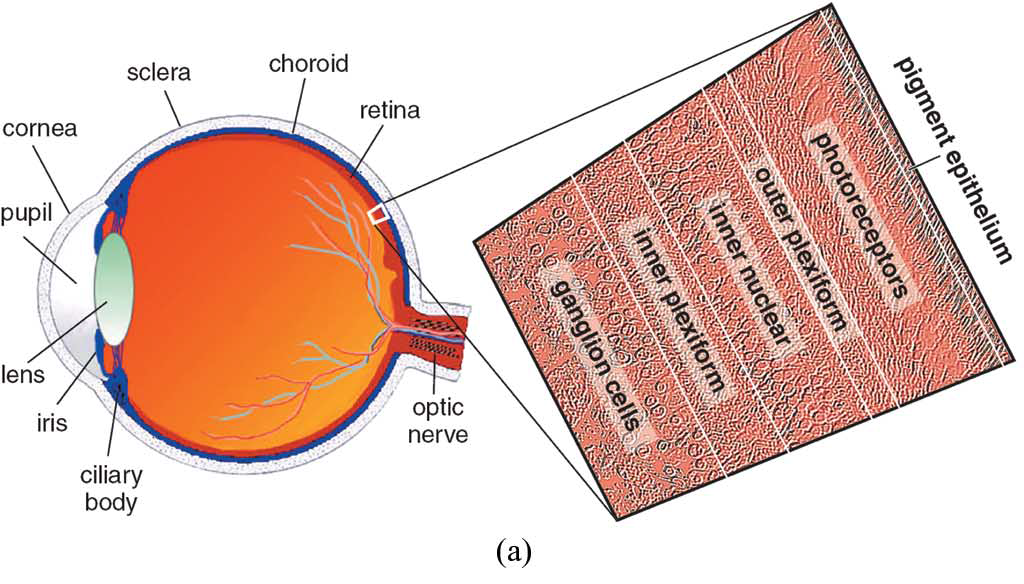
\includegraphics[height=5cm]{./Figures/retina_a.png}
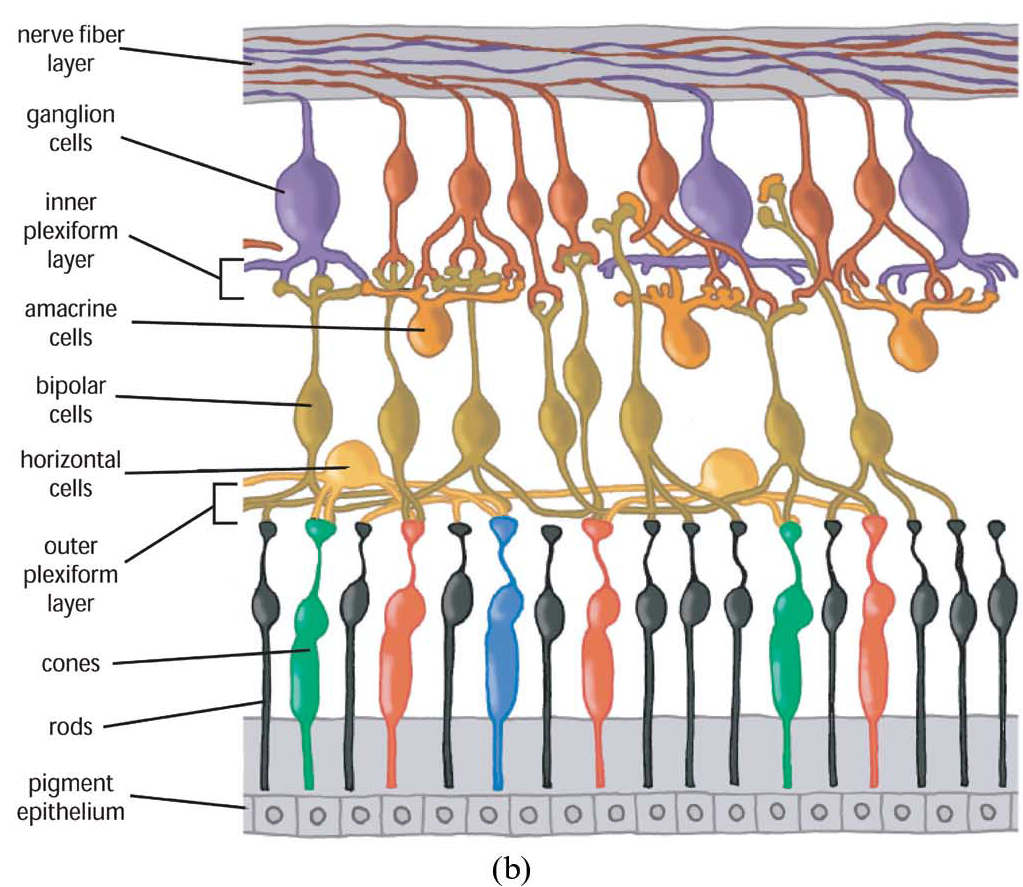
\includegraphics[height=5cm]{./Figures/retina_b.png}
\label{fig:retina}
\caption{( A) lustración de la anatomía del ojo y capas de la retina  Vista de la sección transversal
del ojo y sus estructuras principales. ( B ) Representación esquemática de las capas celulares de la retina}
\end{figure}

			\subsubsection{Enfermedades que la aquejan}
			
Debido a la arquitectura de la retina, se pueden manifestar en esta tanto enfermedades del ojo como aquellas que afectan la circulación y al cerebro. Estas incluyen enfermedades oculares, como son la degeneración macular y el glaucoma, las cuales son la 1er y 3er causas más importantes de ceguera en el mundo desarrollado. Algunas enfermedades sistémicas también pueden afectar la retina. Complicaciones de tales enfermedades pueden ser retinopatía diabética de la diabetes, la segunda causa más importante de ceguera en el mundo desarrollado, retinopatía hipertensiva desde las enfermedades cardiovasculares, y la esclerosis múltiple. Entonces, por un lado, la retina es sensible a enfermedades específicas del órgano y sistémicas, y por el otro, la captura de imágenes de la misma permite detectar, diagnosticar y controlar enfermedades propias del ojo como así también complicaciones de la diabetes, hipertensión y otras enfermedades cardiovasculares.
			



A continuación una breve reseña de las enfermedades más relevantes que pueden ser estudiadas a través de la captura y el análisis de imágenes del ojo.

\begin{description}
    \item[Diabetes:] Diabetes melitus, de acuerdo a la actual definición de la Organización Mundial de la Salud, es típicamente diagnosticada si un paciente en ayuna tiene un nivel de glucosa plasmática superior a 7.0 mmol/l. Sus causas no se comprenden por completo, pero la herencia genética, la obesidad, y un estilo de vida sedentario incrementan el riesgo de desarrollar diabetes. Los tratamientos consisten principalmente en cambios de dieta, administración de insulina y/o drogas anti-hipoglucémicas. Se sabe que la hiperglucemia, presencia elevada de glucosa en la sangre, daña los vasos sanguíneos cortos y largos, como también células nerviosas, por lo que daña los riñones, el corazón, el cerebro y los ojos, resultando en una complicación de la retina llamada retinopatía diabética.
    \item[Retinopatía diabética:] La retinopatía diabética (DR) es una complicación de la diabetes melitus y la segunda causa más común de ceguera y pérdida visual en U.S., y la más importante causa en la población en edad de trabajo. El número de pacientes con diabetes en U.S., está incrementando rápidamente y en 2007 alcanzó 23.5 millones. Hay una abundante evidencia de que la ceguera y la pérdida visual en estos pacientes puede ser prevenida a través de exámenes anuales y  diagnóstico temprano. En los ojos, la hiperglucemia daña las paredes de los vasos de la retina, la cual puede llevar a:
Isquemia, resultando en el crecimiento de nuevos vasos sanguíneos, los cuales pueden subsecuentemente sangrar y/o causar desprendimiento de la retina, condición llamada retinopatía diabética proliferativa;
caída de la barrera sangre-retina, conduciendo a derrames, edema macular diabético (DME) y daños en los fotorreceptores.
La causa principal de pérdida visual en personas con diabetes es DME, la cual es la más común en diabetes de tipo 2. La caída de la barrera sangre-retina causa el derrame de los capilares dilatados hiper permeables y microaneurismas hacia los tejidos de la rutina intracelular y extracelular con una subsecuente acumulacion de fluido. El edema macular clínicamente significativo ocurre si hay espesamiento de la retina involucrando el centro de la retina o el área en un radio de 500 um, si hay exudaciones fuertes en o dentro de 500 um del centro con espesamiento de la retina adyacente, o si hay una zona de espesamiento de la retina con una área igual o mayor al disco óptico, cualquier parte dentro del diámetro del disco de la retina. Esta definición del CSME generalmente hace referencia al nivel de umbral en el cual se considera realizar un tratamiento de fotocoagulación con láser. Mientras la pérdida visual ocurre cuando el edema macular involucra el centro visual, en menor grado DME puede causar deterioramiento visual.
Está claro que DME afecta la estructura macular tanto a corto como a largo plazo. El derrama exudado en DME inicialmente entra en el citoplasma de las células de Muller, preferencialmente en la retina externa, aunque se ha encontrado que la acumulacion de fluido se extiende través de la mayoría de las capas maculares en etapas más avanzadas de DME. Los quistes predominantemente ocurren en la retina externa. A través del tiempo, los quistes tienden a explotar (fundirse ) y extenderse desde el exterior al interior de la retina. En estos casos, se produce atrofia o apoptosis en el tejido restante de la retina. Serios desprendimientos pueden ocurrir en el 20\% de los casos de DME y no parece correlacionarse con agudeza visual. Exudaciones fuertes pueden ocurrir y tienden a estar ubicadas en el nivel de la capa plexiforme externa. Pacientes que hace tiempo tienen DME con disminución de agudeza visual muestran sensibilidad direccional de los fotorreceptores y densidad pigmentaria visual disminuidas.
El control de la diabetes principalmente involucra la reducción de azúcar en sangre, a través de dietas, cambios en el estilo de vida y drogas antidiabéticas. Si DR está presente,  el control de CSME y DR proliferativa a través de fotocoagulación con láser, la administración de factores de crecimiento anti-vascular, y de los esteroides se ha demostrado en ensayos clínicos aleatorios para prevenir la ceguera y la pérdida visual.
    \item[Degeneración macular asociada a la edad(AMD, age-related macular degeneration):]La degeneración macular asociada a la edad es la causa más común de pérdida visual en los Estados Unidos y es un problema en crecimiento de la salud pública. Actualmente, casi 7.3 millones de Norteamericanos (6.12\% de los Norteamericanos de 40 o más años) tiene alguna clase de AMD, y la AMD es la causa de ceguera del 54\% de las personas ciegas de Norteamerica. La AMD severa reduce la probabilidad de obtener empleo en un 61\% y el salario en un 39\%, mientras que la AMD leve reduce estos en un 44\% y 32\% respectivamente. El costo anual generado por la AMD en los Estados Unidos se estima en 30 billones. Se espera que la incumbencia de la AMD se duplique en los siguientes 25 años. Las dos formas mas prevalecientes son la AMD húmeda y la AMD seca, de las cuales la segunda típicamente conlleva a una pérdida de la agudeza visual gradual. La AMD húmeda, también llamada neurovascularización coroidal (CNV), es la amenza visual mas importante, caracterizada por el crecimiento interno de la estructura vascular coroidal hacia la macula acompañado por un incremento en la permeabilidad vascular. El incremento en la permeabilidad vascular lleva a un agrupamiento anormal de fluidos dentro o por debajo de la retina que causa disfunción visual cuando involucra el centro de la mácula. El curso natural de la CNV es el rápido deterioro de la agudeza, cicatrices en el epitelio pigmentario, y pérdida visual permanente o ceguera. El progreso de la AMD seca puede ser aminorado en muchos pacientes a través de suplementos dietarios, mientras que la pérdida visual por la AMD húmeda es tratada con administración intravítrea de factor de crecimiento anti-vascular.
     
     
\item[Malaria Cerebral:]La Malaria Cerebral (MC) es la mayor causa de muerte y discapacidad, especialmente en chicos en África subsahariana. MC es caracterizada por una secuencia de parásitos eritrocitos
en los vasos cerebrales pero a pesar de la mucha  investigación, los mecanismos por los que el parásito de la malaria intravascular causa coma y la muerte siguen sin estar claros.
La retinopatía  malaria (RM) ha sido identificada como un signo clínico importante en el diagnostico y pronostico de la malaria cerebral. La retina y el cerebro son afectados de forma similar en la MC, y así las características fotográficas de RM son propensas a dar una valiosa información adicional sobre el proceso , diagnóstico , tratamiento y pronóstico de la enfermedad en MC.

     
     \item[Enfermedades cardiovasculares:] Las enfermedades cardiovasculares se manifiestan en la retina de diferentes maneras. La hipertensión y la arteriosclerosis causan cambios en la relación entre el diámetro de las arterias y de las venas de la retina, conocido como relación arteria/vena. Una caída en la relación A/V, por ejemplo, adelgazamiento de las arterias y engrosamiento de las venas, está asociado con un riesgo de accidente cerebro-vascular o infarto en el miocardio. La hipertensión puede también involucrar isquemia en la retina, lo que causa infartos en la misma que se ven como copos de algodón e infartos en la coroide que son visibles como puntos blancos profundos. Además, las enfermedades vasculares sistémicas pueden causar oclusiones arteriales y venosas, conocidas como oclusiones arteriales centrales y de brazos y oclusiones venosas centrales y de brazos. \cite{fraz2012blood}
\end{description}






			\subsubsection{Modalidades de imagen}



Existen varias modalidades de imágenes que permiten analizar el ojo. A continuación se describirán entre los métodos más comunes: el método de captura, elementos necesarios, si son o no invasivas al organismo y su costo.

\begin{description}
\item[Fondo de ojo:] Para realizar la captura del fondo de ojo, se dilata la pupila con fármacos que se depositan en forma de gotas en la superficie ocular; así, el oftalmólogo puede ver con facilidad el interior del globo ocular con un aparato que se llama oftalmoscopio. Esta modalidad no es invasiva, y su costo es menor a la angiografía y la OCT dado que la cámara que se necesita para capturar la imagen del ojo es una cámara digital convencional.

\item[Angiografía Fluorescente:] La secuencia de angiogramas fluorescentes involucra la inyección de un tinte fluorescente por vía intravenosa, las luz irradiada por este tinte es capturada por una c\'amara diseñada para este prop\'osito. Diferentes porciones de la vasculatura se vuelven visibles en diferentes momentos, a medida que el tinte pasa a través del sistema vascular.  Esta modalidad es invasiva dado que requiere la inyección de  un tinte fluorescente en el organismo, y es más costoso debido a que se requiere un dispositivo que capte la fluorescencia generada por el tinte inyectado.


\item[OCT:] El OCT es una técnica de imagen tomográfica óptica que permite visualizar tejidos oculares con un nivel de resolución micrométrico, diez veces mayor que al alcanzado por técnicas ultrasonográficas. Esto permite apreciar cambios sutiles de los diferentes tejidos del ojo casi a nivel celular, permitiéndonos entender mejor los procesos patológicos subyacentes a diferentes enfermedades y ayudándonos en el diagnóstico de patologías oculares, principalmente de la retina y el nervio óptico. 
Esta tecnología se basa en un principio óptico complejo denominado interferometría, que utiliza una fuente de luz infrarroja que penetra en los tejidos oculares y se divide en varios haces de luz. Uno de ellos penetra en la retina y otro es captado por un espejo de referencia. En su trayectoria de regreso, ambos haces chocan entre sí generando unas “interferencias” que al ser captadas por un detector se traducen en una imagen en color que representa e indica el grosor de las de los tejidos estudiados. Los colores fríos, como el azul o el negro, se correlacionan con tejidos de menor grosor y los colores cálidos, como el rojo o blanco, con tejidos más gruesos.
Esta modalidad no es invasiva, pero su costo es bastante mayor a la imagen de fondo de ojo, dado que utiliza un tom\'ografo para realizar el proceso.
\end{description}

	\subsubsection{Angiograf\'ias con fluoresce\'ina}

	
Desde su introducci\'on en 1960, la angiograf\'ia fluorescente ha sido una herramienta fundamental en el diagn\'ostico y tratamiento de enfermedades de la retina, a menudo ofreciendo una idea de la presencia, actividad y gravedad de enfermedades no apreciables a trav\'es de solo la examinaci\'on cl\'inica.\cite{patel2014ultra}
\\

La fluorescencia es la propiedad de ciertas mol\'eculas de emitir luz de una longitud de onda superior cuando son
estimuladas por una luz de menor longitud de onda. El pico de excitaci\on de la fluoresce\'ina es de, aproximadamente, 490 nm (en la parte azul del espectro) y representa la m\'axima absorci\'on de energ\'ia lum\'inica por la fluoresce\'ina. Las mol\'eculas estimuladas por esta longitud de onda son excitadas hasta un nivel de energ\'ia superior y emiten luz de aproximadamente 530 nm \ref{fig:wavechanges1}.


%\begin{figure}[H]
%\centering
%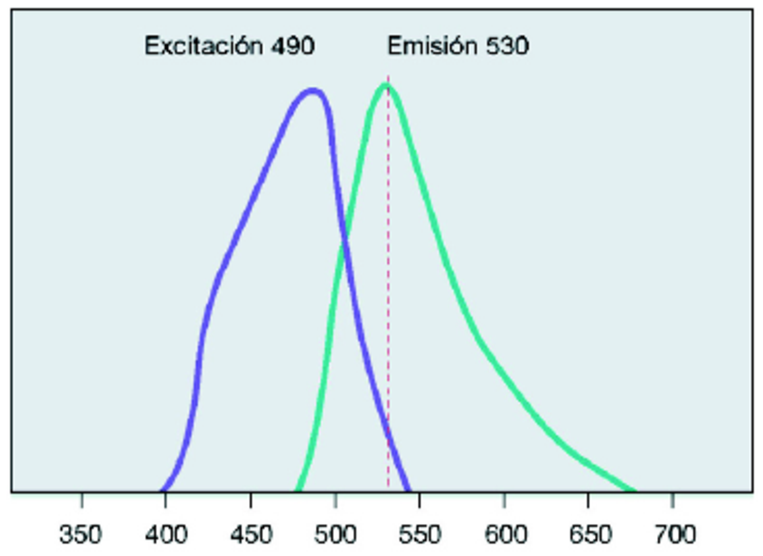
\includegraphics[height=5cm]{./Figures/wavechanges.pdf}
%\label{fig:wavechanges}
%\caption{ Longitud de onda en los estados de exitaci\'on y emisi\'on de la fluoresc\'ina.}
%\end{figure}


\begin{figure}[H]
  \centering
	\begin{subfigure}[b]{0.45\textwidth}
        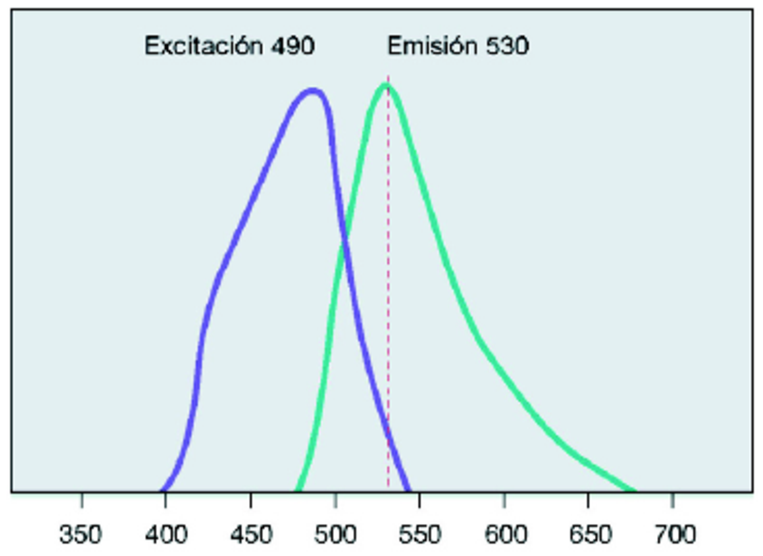
\includegraphics[width=1\textwidth]{./Figures/wavechanges.pdf}
        \caption{Longitud de onda en los estados de exitaci\'on y emisi\'on de la fluoresc\'ina.}
        \label{fig:wavechanges1}
    \end{subfigure}
	\begin{subfigure}[b]{0.45\textwidth}
        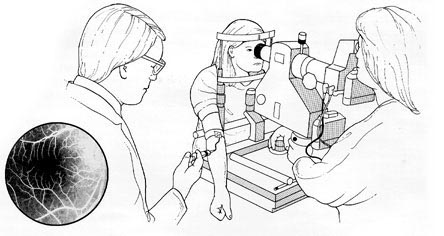
\includegraphics[width=1\textwidth]{./Figures/fluores.jpg}
        \caption{Proceso de administraci\'on de la fluoresce\'ina.}
        \label{fig:af2}
    \end{subfigure}
    \caption{Administraci\'on y reacci\'on de la fluoresce\'ina.}
\end{figure}



Durante la captura de las angiograf\'ias fluorecentes se le administran al paciente gotas oculares que hacen dilatar la pupila. Se debe colocar la barbilla sobre un apoya-ment\'on y la frente contra una barra de soporte para mantener la cabeza quieta durante el examen. Se toman fotograf\'ias del interior del ojo . Despu\'es de tomar el primer grupo de im\'agenes, se inyecta un tinte llamado fluoresce\'ina, dentro del  torrente sangu\'ineo. En la mayor\'ia de los casos, se inyecta en la parte interior del codo. Un dispositivo similar a una c\'amara, denominada angi\'ografo, toma fotograf\'ias a medida que el tinte va pasando a lo largo de los vasos sangu\'ineos en la parte posterior del ojo. El contenido sangu\'ineo mezclado con la fluoresce\'ina produce una emisi\'on intensa de luz que permite el registro fotogr\'afico de los vasos de la retina y las coroides. Proporciona excelentes im\'agenes del \'arbol vascular.

%\begin{figure}[H]
%\centering
%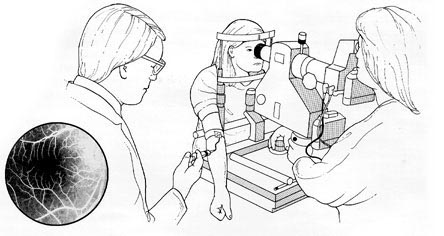
\includegraphics{./Figures/fluores.jpg}
%\label{fig:retina}
%\caption{( A) lustración de la anatomía del ojo y capas de la retina  Vista de la sección transversal
%del ojo y sus estructuras principales. ( B ) Representación esquemática de las capas celulares de la retina}
%\end{figure}

Se utilizan filtros de dos tipos para asegurarse de que la luz azul entra en el ojo y s\'olo la luz amarillo-verde entra en la c\'amara (\ref{fig:lightfilter}).
\begin{description}
  \item[a.] 
 Filtro de excitaci\'on de azul cobalto que permite el paso la luz blanca desde la c\'amara. La luz azul emergente
entra en el ojo y excita las mol\'eculas de fluoresce\'ina en las circulaciones retiniana y coroidea, que luego emiten
luz de una mayor longitud de onda (amarillo-verde).
\item[b.] A continuación, un filtro de barrera amarillo-verde bloquea cualquier luz azul reflejada del ojo, y permite
únicamente el paso de la luz fluorescente amarilloverde emitida.\cite{kanski2012oftalmologia}
\end{description}


poner img
\begin{figure}[H]
\centering
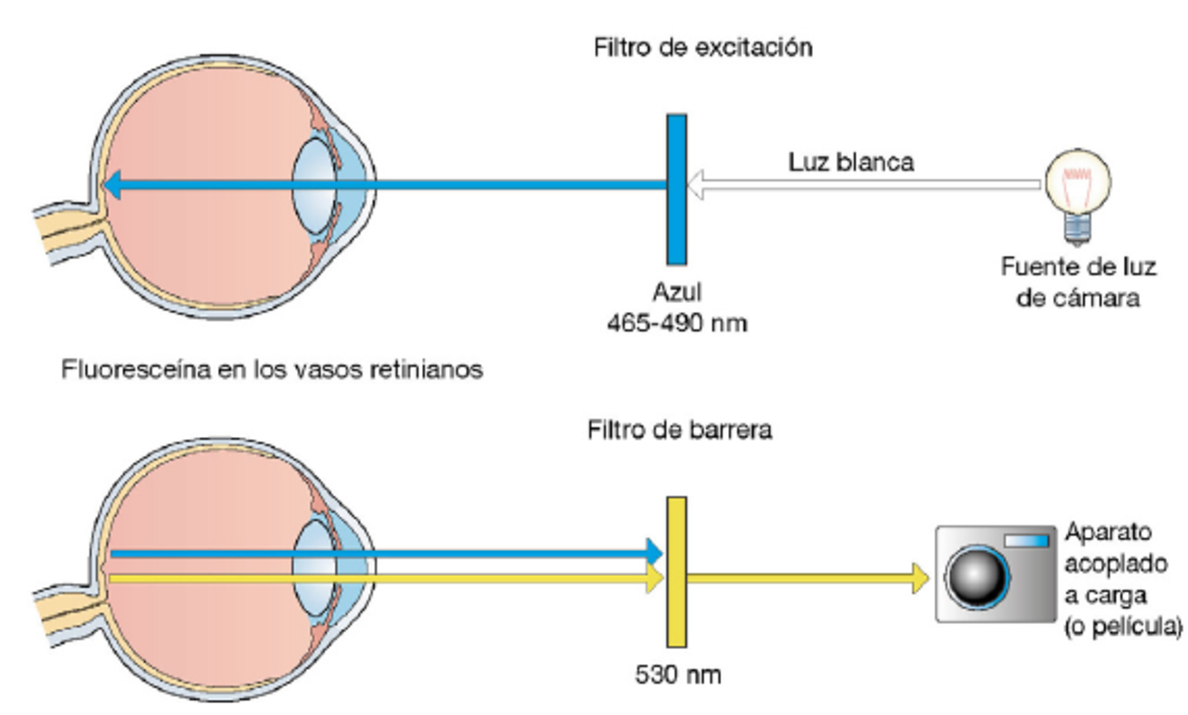
\includegraphics[width=0.9\textwidth]{./Figures/filtrosluz.pdf}
\label{fig:lightfilter}
\caption{ Bla bla bla bla}
\end{figure}



La angiograf\'ia con fluoresce\'ina presenta varias peculiaridades. El desaf\'io principal es que, a medida que el tinte de contraste  perfunde en la retina, diferentes segmentos de la vasculatura aparecen, por lo que el contenido de la imagen var\'ia constantemente.
Pueden ocurrir oclusiones debido a los p\'arpados y las pestañas, algunas lesiones pueden parecerse a los vasos creando falsos positivos y los vasos perif\'ericos aparecen a menudo distorsionados y difusos. \cite{perez2011improving}

Conociendo los tiempos en los que se llenan las diferentes partes de la red vascular y teniendo fotograf\'ias consecutivas, el oftalm\'ologo logra hacer un mapa del fondo ocular permitiendo detectar con facilidad: anormalidades en el curso de los vasos sangu\'ineos; defectos estructurales de sus paredes; aparición de nuevos vasos; e incipientes desprendimientos de la retina. 

La indicaci\'on más habitual es el estudio de problemas vasculares y, en concreto, la retinopat\'ia diab\'etica, as\'i como en patolog\'ias maculares como la Degeneraci\'on macular asociada a la edad con el fin de diagnosticar si hay presencia o no de una membrana neovascular.
\\

\begin{figure}[H]
  \centering
	\begin{subfigure}[b]{0.23\textwidth}
        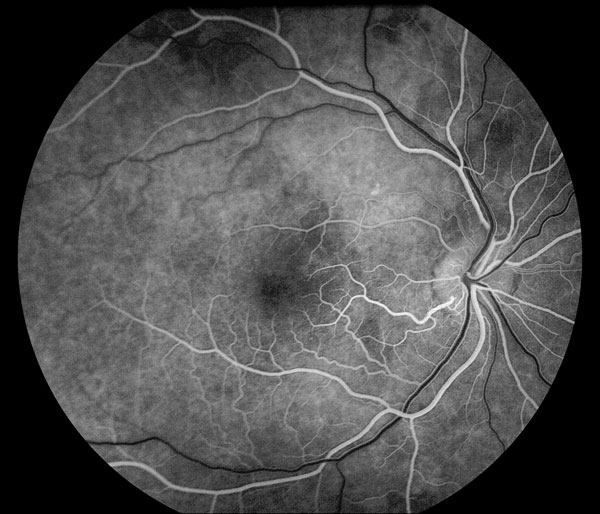
\includegraphics[width=1\textwidth]{./Figures/FA_Fig1.jpg}
        \caption{Time 0}
        \label{fig:af1}
    \end{subfigure}
	\begin{subfigure}[b]{0.23\textwidth}
        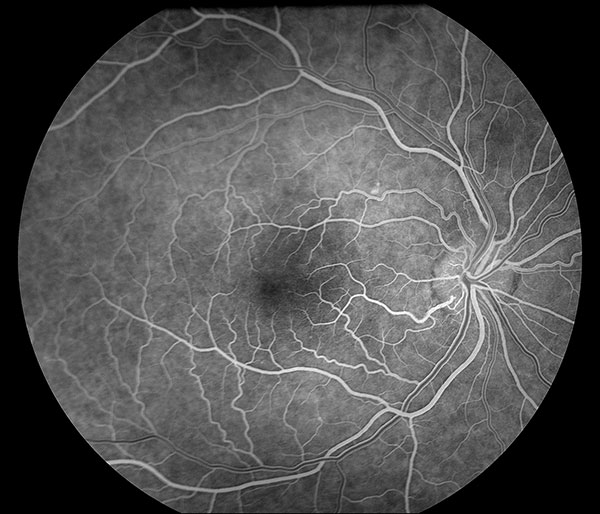
\includegraphics[width=1\textwidth]{./Figures/FA_Fig2.jpg}
        \caption{Time 1}
        \label{fig:af2}
    \end{subfigure}
	\begin{subfigure}[b]{0.23\textwidth}
        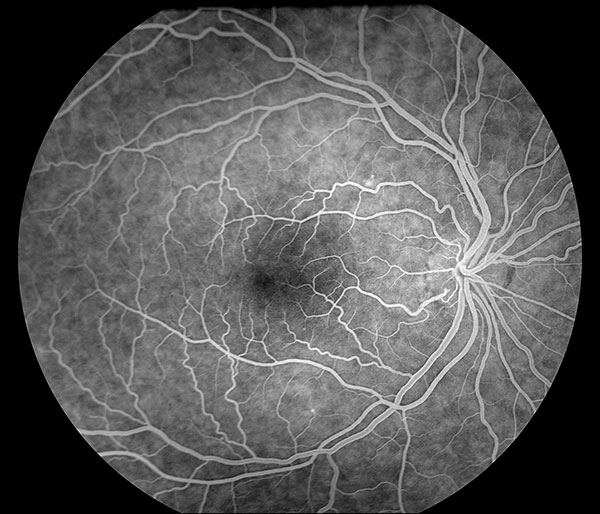
\includegraphics[width=1\textwidth]{./Figures/FA_Fig3.jpg}
        \caption{Time 2}
        \label{fig:af3}
    \end{subfigure}
    	\begin{subfigure}[b]{0.23\textwidth}
        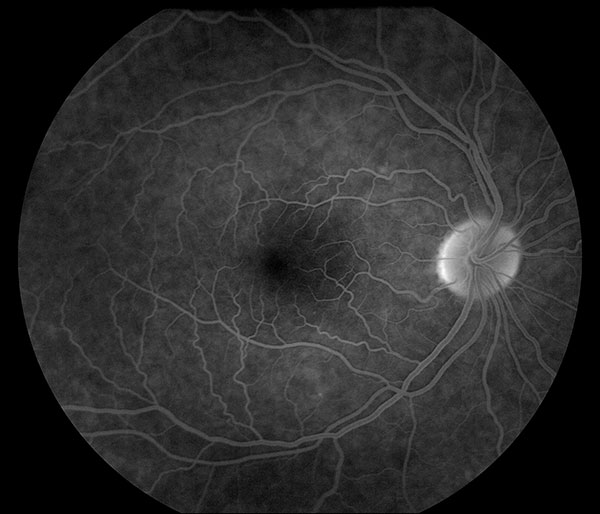
\includegraphics[width=1\textwidth]{./Figures/FA_Fig4.jpg}
        \caption{Time 3}
        \label{fig:af4}
    \end{subfigure}
	\label{fig:retina}
	\caption{Angiograf\'ia con fluoresc\'ina}
\end{figure}


	\subsection{Angiograf\'ias con fluoresce\'ina de amplio ángulo}

Como muchas enfermedades de la retina se manifiestan con anormalidades periféricas, ha habido una presión cada vez mayor para mejorar la captura de im\'agenes de la periferia de la retina. 
Tradicionalmente el fondo de ojo ofrece un campo de visi\'on que va desde los 30\degree a 60\degree en una exposición. La examinación de la periferia de la retina requiere habilidades técnicas del fotógrafo como la redirección de la mirada por parte del paciente, e incluso as\'i la periferia lejana no es fotografiada.
La angiografía de amplio ángulo con el uso de lentes de contacto expande la vista a 150\degree-160\degree pero es técnicamente más desafiante y requiere de la cooperación del paciente con el lente de contacto. 
El Optos Optomap Panoramic 200A imaging system (Optos, PLC, Scotland) promueve el ensanchado del campo de visión a 200\degree. El sistema  Optos Optomap Panoramic usa una tecnología de escáner láser oftalmoscopio con un espejo en forma de elipsoide, formando un escaneo que cubre el 82\% de la retina en  una simple imagen.
La Angiografía  fluorescente ultra-wide-field (UWFA), se describió por primera vez en 2004 por Friberg y Forrester, no sólo captura un campo ancho de la retina de una sola vez  permitiendo la visualización de diferentes áreas de la retina  al mismo  tiempo durante la angiografía y reduciendo la cantidad de cooperación del paciente y la experiencia técnica requerida por el fotógrafo, sino también visualiza la periferia de la retina que antes no podía ser fotografiado. Comparado con los sistemas de adquisición digital convencional, UWFA captura el doble de área de la retina.
\\
La angiografía con fluoresceína es fundamental para la tratamiento de la retinopatía diabética, ya que en esta se pueden detectar microaneurismas, no perfusión, edema macular y neovascularización. A pesar de que las anormalidades de la retinopatía diabética, especialmente la no perfusión, pueden ocurrir en la periferia media o la periferia, la captura de imágenes ultra-wide-field puede ser particularmente útil en la evaluación de estas condiciones.\cite{patel2014ultra}	


\begin{figure}[H]
	\centering
	\begin{subfigure}[b]{0.23\textwidth}
        \includegraphics[width=1\textwidth]{./Figures/AF1.png}
        \caption{Time 0}
        \label{fig:af1}
    \end{subfigure}
	\begin{subfigure}[b]{0.23\textwidth}
        \includegraphics[width=1\textwidth]{./Figures/AF2.png}
        \caption{Time 1}
        \label{fig:af2}
    \end{subfigure}
	\begin{subfigure}[b]{0.23\textwidth}
        \includegraphics[width=1\textwidth]{./Figures/AF3.png}
        \caption{Time 2}
        \label{fig:af3}
    \end{subfigure}
    	\begin{subfigure}[b]{0.23\textwidth}
        \includegraphics[width=1\textwidth]{./Figures/AF4.png}
        \caption{Time 3}
        \label{fig:af4}
    \end{subfigure}
	\label{fig:retina}
	\caption{Angiograf\'ia con fluoresc\'ina}
\end{figure}


\subsubsection{AF para detecci\'on enfermedades }

explicar en qué contextos se las usan, para el diagnóstico de cuáles enfermedades, y qué cosas se ven en ellas.

MALARIA CEREBRAL
Los Intravascular filling defects (IVFD) son características de  MR que pueden ser observadas en imágenes de  angiografías de fluorescencia (AF) .IVFD puede representar secuencias de parásitos eritrocitos en la microvasculatura. Sequestration es la característica patológica de la malaria cerebral , pero hasta ahora , sólo ha sido posible cuantificar histopatológicamente en el post mortem . IVFD puede ser visto en pequeñas y largas vénulas arteriolas y los capilares , pero parecen ser más prominente en las vénulas. Sequestration del cerebro y la retina es siempre visto en casos fatales de MC con RM, y la apariencia de la histopatología es similar en IVFD. Además, IVFD a menudo resuelve el dia despues del tratamiento con medicamentos contra la malaria. Esto es consonancia con  la resolución de sequestration y la recuperación clínica. Es plausible que  IVFD representa proceso patológico fundamental, y esta lesión merece una mayor investigación. \cite{zhao2015automated}

IMAGEN

\textbf{Edema Macular Diabético}

La angiografía de fluorescencia es una poderosa herramienta para la captura de imagenes y evaluación del edema macular diabético (EMD). donde el tinte fluorescente se acumula en las áreas enfermas.
El EMD es un proceso patológico que consiste en la anormal permeabilidad de la retina que resulta en la fuga y acumulación de fluidos en la capa de la retina del ojo. Es definido como la presencia de engrosamiento de la retina que involucra la mácula, definida como el área a 2 discos ópticos de distancia desde el centro de la visión (ej. fóvea ). El resultado es la visión borrosa en el paciente y puede conducir a la deficiencia visual en etapas adelantadas si no se trata. \cite{el2011segmentation}

IMAGEN

El Edema Macular Diab\'etico, en particular, es un gran contribuyente a la p\'erdida de la visi\'on  entre pacientes con Retinopat\'ia Diab\'etica. Hace m\'as de 25 a\~nos, el Early Treatment of Diabetic Retinopathy Study (ETDRS) estableci\'o gu\'ias para identificar los edemas maculares cl\'inicamente significativos y prob\'o que el tratamiento con fotocoagulaci\'on con laser focal decrementa el riesgo de perdida moderada de la visi\'on, incrementa las posibilidades de ganancia visual moderada y reduce el engrosamiento retinal. \textbf{While ETDRS remains the seminal study on DMO, additional awareness of diabetic pathology,} el advenimiento de la nueva farmacolog\'ia y las mejoras en la tecnolog\'ia de captura de im\'agenes de la retina nos han permitido expandir nuestro entendimiento y tratamiento del edema macular diab\'etico.
Hace tiempo se ha hipotetizado que los cambios isqu\'emios y las patolog\'ias microvasculares  juegan un papel en el desarrollo del Edema Macular Diab\'etico. En la Retinopat\'ia Diab\'etica, la isquemia estimula la producci\'on de factor de crecimiento vascular endotelial(VEGF, por sus siglas en ingl\'es), lo que puedo conducir al quiebre de las barreras sangre-retina, y puede causar Edema Macular Diab\'etico por incremento de la permeabilidad de los vasos sangu\'ineos. Las drogas Anti-VEGF han probado eficacia en el tratamiento del Edema Macular Diab\'etico, incluso en los casos que no responden a la fotooagulaci\'on por laser. El \'exito de la terapia anti-VEGF da sustento a la idea de que la isquemia retinal y el Edema Macular Diab\'etico est\'an asociados, pero la captura de im\'agenes de retinal tradicional dificulta el estudio de esta asociaci\'on.
La isquemia retinal se caracteriza mejor utilizando angiograf\'ias fluorescentes(FA). Las FA tradicionales emplean fotograf\'ia retinal que es capaz de ver aproximadamente 30\degree de la retina por im\'agen. El ETDRS desarrollo el protocolo \textbf{the seven-standard fields (7SF)} en donde 7 \'areas de la retina fotografiadas son combinadas para dar una visualizaci\'on cercana a 75\degree. Con el advenimiento de las angiograf\'ias fluorescentes de ultra campo de visi\'on (UWFA), as\'i como de los sistemas de captura Optos 200Tx, es ahora posible ver 200\degree de la retina en una sola fotograf\'ia. Los estudios a peque\~na escala iniciales mostraron que las UWFA son m\'as \'utiles en la detecci\'on de la no perfusi\'on de capilares en pacientes con Edema Macular Diab\'etico que otros m\'etodos con campos de visi\'n m\'as limitados en la captura de im\'agen.\citep{wessel2012peripheral}

	\subsection{Herramientas computacionales para an\'alisis de agiograf\'ias con fluoresce\'ina}



\section{Segmentaci\'on de vasos sangu\'ineos en FA}

	\subsection{Necesidad}
	La retinopatía diabética ( RD) es el líder en las patologías oftalmológicas y causante de ceguera entre las personas en edad de trabajar en los países desarrollados . Está provocada por complicaciones en la diabetes mellitus y , aunque los efectos de la diabetes no necesariamente implican el deterioro de la visión , el 2\% de los pacientes afectados por este trastorno son ciegos y el 10\% padecen  degradación de la visión después de 15 años de diabetes como consecuencia de complicaciones RD . La prevalencia estimada de diabetes por todos los grupos de edad en todo el mundo fue de 2,8\% en 2000 y 4,4\% en 2030 , lo que significa que el número total de pacientes con diabetes se prevé aumente de 171 millones en el  2000 a 366 millones en el 2030 .
	A pesar de que la RD es una enfermedad incurable, la fotocoagulación láser puede prevenir la pérdida de la visión si es detectada en etapas tempranas. Sin embargo, los pacientes con RD no perciben ningún síntoma hasta que la pérdida de visión se desarrolla, por lo general en estadios de la enfermedad más adelantados, cuando el tratamiento es menos eficaz. Entonces, para garantizar que el tratamiento es recibido a tiempo, los pacientes diabéticos necesitan un examen anual de fondo de ojo. Sin embargo, esta acción preventiva involucra un enorme desafío para el Sistema de Salud debido  al gran número de pacientes que necesitan revisión oftalmológica. Por lo tanto, la RD también llega a ser un gran problema económico en la  Administración Pública ya que ,solo en U.S, el costo de las complicaciones oftalmológicas crónicas causada por la diabetes excedió un billón de dólares en 2007.
El uso de imágenes digitales para diagnosticar enfermedades del ojo podría ser explotado por sistemas de computadora para la detección temprana de RD. Un sistema que podría ser  usado por personal no experto para filtrar casos de pacientes no afectados por enfermedades, haría reducir la carga de trabajo del especialista e incrementaria la efectividad de los protocolos de prevención y os tratamientos terapéuticos en etapas tempranas. Además, esto sería también un resultado beneficio en el Sistema de Salud, ya que el costo-efectividad asociado a la detección temprana de enfermedades da lugar a un ahorro de costos notables.
Ya que las anomalías vasculares son una de las manifestaciones de la RD, la evaluación automática de los vasos sanguíneos de fondo de ojo es necesario para automatizar la detección de RD. Como un paso previo, la evaluación de los vasos demanda la segmentación del árbol vascular para su posterior procesamiento. El conocimiento de la ubicación de los vasos sanguíneos para reducir el número de falsos positivos en la detección de microaneurismas y hemorragias. Además, estas aplicaciones motivadas por la automática detección temprana de RD, la segmentación del árbol vascular resulta útil para otros propósitos clínicos: evaluación de retinopatía prematura, estrechamiento arterial, tortoise en los vasos para caracterizar retinopatía hipertensiva, medida del diámetro de los vasos para diagnosticar hipertensión y enfermedades cardiovasculares y cirugía láser por computación asistida, entre otras.
Por otro lado, el árbol vascular también sirve para ser usado como información valiosa para ubicar otras características del fondo de ojo como el disco óptico y la fóvea. \cite{marin2011new}

	\subsection{M\'etodos existentes}



	\subsubsection{Supervisados}

En los m\'etodos supervisados, la regla para extracci\'on de vasos es aprendida por un algoritmo en base a un conjunto de im\'agenes de referencia manualmente procesadas y segmentadas generalmente llamadas estandar de oro. Estas estructuras vasculares en dichas im\'agenes son marcadas con presici\'on por un oftalmologo. Sin embargo, como menciona Hoover et al. \cite{hoover2000locating} existe un desacuerdo significativo en la identificaci\'on de vasos incluso entre observadores expertos. En un m\'etodo supervisado, el criterio de clasificaci\'on es determinado por los datos de referencia basados en las caracter\'isticas seleccionadas. Por lo tanto el pre-requisitos es la disponibilidad de im\'agenes de referencias clasificadas, las cuales muchas veces no est\'an disponibles en aplicaciones de la vida real. Como estos m\'etodos est\'an dise\~nados basados en datos pre-clasificados, su desempeño es generalmente mejor que aquellos que no son supervisados y pueden producir muy buenos resultados para im\'agenes "saludables" de la retina.

	\subsubsection{No supervisados}


Los enfoques basados en clasificaci\'on no superviada intentan encontrar los patrones inherentes a los vasos sang\'ineos de las im\'agenes de la retina que pueden ser utilizados para determinar si un pixel en particular pertenece o no a un vaso. Los datos de referencia no contribuyen directamente al dise\~no del algoritmo en estos enfoques.

En general, existen tres principales desafios que deben abordarse en el automatizado de la segmentación de vasos de la retina :
\begin{enumerate}
\item La calidad de imagen es a menudo un problema de interés para el desarrollo de la segmentación automatizada. Técnicas de segmentación existentes todavía se enfrentan a desafíos en la segmentación de toda la vasculatura con precisión , debido al poco contraste, fondos no homogéneos y la presencia de ruido durante la adquisición de imagen.
\item La complejidad de la estructura vascular (por ejemplo, múltiples escalas y orientaciones), el alto grado de variación anatómica a través de la población y la complejidad de los tejidos / órganos de alrededores
, plantean desafíos significativos en segmentación de los vasos. El realce de los vasos es
una forma efectiva para facilitar la segmentación:  pero comúnmente usar filtros de realce no es en términos de rendimiento.
\item Un eficiente y robusto modelo de segmentación  es deseable. Se ha vuelto muy difícil
para elegir un modelo óptimo, o para identificar un único conjunto de parámetros óptimos para un método de segmentación en particular que trabaje a través de una variedad de datos.\cite{zhao2015retinal}
\end{enumerate}



\subsubsection{métodos de segmentación en FA}
*****métodos de segmentación en FA******

\subsubsection{papelera}
La vasculatura retinal está compuesta por arterias y venas que aparecen como estructuras alargadas, con sus afluentes visibles dentro de la imagen de la retina.
Los anchos de los vasos son muy variados y van de uno a veinte pixels dependiendo del ancho del vaso y de la resolución de la imagen.
\\
La orientación y nivel de gris de los vasos no cambia abruptamente, son localmente lineales y cambian gradualmente en intensidad a lo largo de su longitud. Los vasos pueden estar conectados y, en la retina, formando una estructura similar a un árbol binario. Sin embargo, la forma, el tamaño y el nivel local de gris de los vasos sanguíneos puede variar enormemente.
\\
La detección automática de enfermedades y el análisis de imagenes de la vasculatura   puede asistir en la implementación de programas de detección de retinopatía diabética, evaluación de retinopatía precoz, detección de regiones avascular foveal, estrechamiento arterial, la relación entre la tortuosidad de los vasos, retinopatía hipertensiva, la medida del diámetro de los vasos en relación con la hipertensión , la cirugía láser asistida por computadora.\cite{fraz2012blood}\\
 
% Chapter Template

\chapter{M\'etodos} % Main chapter title

\label{Chapter3} % Change X to a consecutive number; for referencing this chapter elsewhere, use \ref{ChapterX}

%----------------------------------------------------------------------------------------
%	SECTION 1
%----------------------------------------------------------------------------------------

\section{Descripci\'on general}

Como se mencion\'o anteriormente, este trabajo se enfoca en extraer informaci\'on sobre los vasos sangu\'ineos oculares en pos de la detecci\'on de enfermedades que pueden reflejarse en los mismos utilizando angiograf\'ias fluorescentes.
Las im\'agenes con fluoresc\'ina carecen de ruido debido a colores y cuestiones \'opticas por su naturaleza, pero a su vez poseen ruido generado por la cantidad de vasos que se encuentra por debajo de la retina en la coroide.\\
Con motivo de realizar un mejor an\'alisis sobre las im\'agenes buscamos, en primer instancia, reducir el ruido de las mismas enfocandonos en realzar los vasos de la retina por sobre los de la coroide. Con esto en mente buscamos algoritmos de preprocesamiento que nos acerquen a lo que buscamos para analizar su comportamiento y poder determinar cual ser\'ia el mas adecuado para preprocesar las im\'agenes antes de extraer la informaci\'on necesaria.

\section{Preprocesamiento}
\subsection{¿Por qu\'e?}
Al analizar los diferentes m\'etodos de captura de la retina podemos observar que en cada una de ellos, aunque en diferentes formas, existe ruido generado por la misma tecnolog\'ia de captura. Para poder lograr un resultado \'optimo debemos ser capaces de llevar el ruido mencionado al nivel m\'inimo posible. Para lograrlo se utilizan distintos algoritmos de preprocesamiento, cada uno de ellos mas o menos eficiente dependiendo del tipo de ruido que exista en la im\'agen.\\
\\
Como objetivos principales del preprocesamiento podemos destacar:
\begin{description}
  \item[Reducci\'on de ruido:] Eliminaci\'on de diferencias de intensidad que son generados por ruido producido generalmente por los elementos de captura de la im\'agen.
  \item[Realce de bordes:] Realzar los bordes para luego facilitar la detecci\'on de los mismos en la etapa de segmentaci\'on.
  \item[Suavizado de im\'agenes:] Permite normalizar las intensidades de los p\'ixeles que estan fuera de la \"normalidad\" del vecindario donde se encuentra.
\end{description}

\subsection{Algoritmos investigados}

Luego de realizar un an\'alisis de investigaci\'on acerca de los algoritmos de preprocesamiento existentes encontramos que aquellos que mejor se adaptaban a las necesidades de nuestra casu\'istica eran aquellos que respetaban los bordes al suavizar la im\'agen.\\
\\
Por un lado analizamos los algoritmos mas adecuados para la eliminaci\'on del fondo de la im\'agen, para este fin decidimos analizar tanto la mediana como la media. Por el otro, buscamos algoritmos para la reducci\'on de ruido para im\'agenes de angiodraf\'ia fluorescente y decidimos quedarnos con el algoritomo de difusi\'on anisotr\'opica[PONER REFERENCIA] y el filtro de coherencia[PONER REFERENCIA].

\subsubsection{Remoci\'on fondo}

Para la remoci\'on de fondo se utilizaron dos filtros diferentes, por un lado el filtro de media y por el otro un filtro de mediana. Tanto la media como la mediana son filtros de paso bajo, es decir, un filtro que aten\'ua las intensidades altas y mantienen las intensidades bajas. Este tipo de filtros intentan reducir el ruido suavizando. En nuestro caso, al ser utilizado con grandes ventanas, nos permiten obtener una imagen homogénea que podemos restar a la imagen original para remover el fondo.

\begin{description}
  \item[Media:] La media, como su nombre lo indica, realiza un promedio entre las instensidades vecinas al p\'ixel llevando a cabo una convoluci\'on y utiliza el resultado para actualizar el valor del mismo.
  \item[Mediana:] Por otro lado, la mediana es un filtro no lineal dado que depende de un algoritmo de ordenamiento para determinar cu\'al es el valor que divide a la mitad al conjunto, al encontrarlo utiliza este para actualizar el valor del p\'ixel analizado.
\end{description}

\subsubsection{Reducci\'on de ruido}

Para la reducci\'on de ruido nos enfocamos en encontrar filtros que nos permitieran suavizar y eliminar ruido pero siempre intentando no perder los borde y objetos de inter\'es de la imagen. Para esto buscamos filtros que puedan orientarse en las direcciones de los bordes y de esta manera mantenerlos con contrastes altos\\
\\En nuestra b\'usqueda encontramos varios algoritmos matem\'aticos que apuntaban en esta direcci\'on como el filtro gaussiano pero determinamos que no estaban plenamente enfocados en mantener las estructuras sino mas bien que esto era una consecuencia de su naturaleza. Sobre el final de la misma, y a trav\'es de la lectura de algunas investigaciones (PONER CITAS) descubrimos el filtro de difusi\'on anisotr\'opica \cite{perona1990scale} y el filtro de coherencia (CITA!!).

\begin{description}
  \item[Difusi\'on anisotr\'opica:]
  \item[Filtro de coherencia:]
\end{description}

\subsection{Resultados obtenidos}

En pos de exponer de manera adecuada los resultados obtenidos de los experimentos realizados proponemos graficar los mismos pero no sin antes explicar como se obtuvieron.\\
\\En todos los casos la metodolog\'ia que se utiliz\'o fu\'e realizar pruebas exhaustivas variando dos par\'ametros: cantidad de iteraciones de los filtros y el tamaño de ventana de la remoci\'o de fondo.\\
\\En ambos casos se relev\'o un rango que se considero suficiente dado que luego de el límite establecido se noto que a grandes pasos los resultados solo deca\'ian en calidad.\\
\\Dada la naturaleza de los experimentos decidimos que la mejor manera de mostrar los resultados era un mapa de calor que podemos ver en la FIGURAX y para poder visualizar mejor el comportameniento en la zona de calor mas intenso aislamos la regi\'on y lo graficamos en tres dimensiones como se puede apreciar en la FIGURAY.\\

FALTAN EXPERIMENTOS:
\begin{description}
  \item[Media con anisodiff] En algun momento descartamos la media pero no tenemos datos guardados para mostrar
  \item[Media con coherencia] En algun momento descartamos la media pero no tenemos datos guardados para mostrar
  \item[Mediana con coherencia] Hicimos el de difusion anistropica, y el de coherencia pudimos buscarle la vuelta ahora para hacerlo mas rapido
\end{description}

\subsection{Comparativa}

Pendiente de los resultados de los experimentos.

\section{Extracci\'on de caracter\'isticas}

\section{M\'etodo de segmentaci\'on}

% Chapter Template

\chapter{Resultados} % Main chapter title

\label{ChapterX} % Change X to a consecutive number; for referencing this chapter elsewhere, use \ref{ChapterX}

%----------------------------------------------------------------------------------------
%	SECTION 1
%----------------------------------------------------------------------------------------

\section{Materiales}

\section{Medidas de calidad}

\section{Configuraci\'on de los experimentos}

\section{Resultados}

\section{Discusi\'on} 
% Chapter Template

\chapter{Conclusi\'on} % Main chapter title

\label{ChapterX} % Change X to a consecutive number; for referencing this chapter elsewhere, use \ref{ChapterX}

 

%----------------------------------------------------------------------------------------
%	THESIS CONTENT - APPENDICES
%----------------------------------------------------------------------------------------

\appendix % Cue to tell LaTeX that the following "chapters" are Appendices

% Include the appendices of the thesis as separate files from the Appendices folder
% Uncomment the lines as you write the Appendices

% Appendix A

\chapter{Appendix Title Here} % Main appendix title

\label{AppendixA} % For referencing this appendix elsewhere, use \ref{AppendixA}

Write your Appendix content here.
%\input{Appendices/AppendixB}
%\input{Appendices/AppendixC}

%----------------------------------------------------------------------------------------
%	BIBLIOGRAPHY
%----------------------------------------------------------------------------------------

\printbibliography[heading=bibintoc]

%----------------------------------------------------------------------------------------

\end{document}  
